\documentclass[10pt]{article}
\usepackage{fullpage}
\usepackage{amsfonts}
\usepackage{amsmath}
\usepackage{amsthm}
\usepackage{graphicx}
\usepackage{color}
\usepackage{amssymb}
\usepackage{empheq}
\usepackage{mathrsfs}
\usepackage{enumerate}
\usepackage{tikz}
\usepackage{pgflibraryarrows}
\usepackage{pgflibrarysnakes}
\usepackage{upgreek}
\usepackage{tipa}
\usepackage{multicol}
\usepackage{verbatim}
\usepackage{floatrow}
\usepackage{gensymb}
\usepackage{caption}

\usepackage{versions}
\excludeversion{sol}
\includeversion{sol}
\newenvironment{solution}{
\sol\\{\sc{Solution:}}}{
$\hfill\blacksquare$\endsol}

\newcommand{\de}[2]{\frac{d #1}{d #2}}

\usepackage[T1]{fontenc}
\usepackage[font=small,labelfont=bf,tableposition=top]{caption}

\DeclareCaptionLabelFormat{andtable}{#1~#2  \&  \tablename~\thetable}



\newfloatcommand{capbtabbox}{table}[][\FBwidth]

\usepackage{fancyhdr}
\setlength{\headheight}{15.2pt}
\pagestyle{fancy}
\setlength\headsep{30pt}
\lhead{Homework 5}
%\chead{\today}
\rhead{MATH 210}

\title{\textbf{\textsc{Homework 5}}\\
Game Theory}
\author{\textbf{\textsc{MATH 210-010 $\diamond$ Fall 2024}}}
%\date{\today}



\begin{document}
\maketitle
\author

\vspace{3cm}
\begin{center}
\textsc{Due: Friday, December 6, 2024 }\\
%\textsc{Read: Matlab Week 1 Handout}
\end{center}


\normalsize
% \fbox{\fbox{\parbox{5.5in}{
 
        {\bf Instructions:}   To complete a problem set, you must submit a zip file labeled \verb|Yourlastname_HW#| to Dropbox no later than 11:59 PM on the due date above.  For example, if I were to complete this assignment, my folder would be named \verb!Emerick_HW5!.  In this folder, a \texttt{py} file is to be submitted for each problem such that when the \texttt{py} file is executed, the output (as presented in Python) is the solution to the problem.  Each \texttt{py} file must be saved as \verb!Yourlastname_HW#_No#.py!.  For example, if I were submitting the answer to Question Number 1 on Homework 5, the \texttt{py} file for that problem would be saved as \verb!Emerick_HW5_No1.py!.  Each \texttt{py} file should be well commented and be free of extraneous lines and commands.  Also, each \texttt{py} file must output only what the problem asked to be outputted.  Failure to abide by these simple homework submission guidelines may result in a deduction of points at my discretion.





%\vspace{4cm}
%\noindent \textsc{Instructions:}  To complete a problem set, you must submit a folder labeled \verb!Yourlastname_PS#! to Dropbox no later than midnight on the due date above.  For example, if I were to complete this assignment, my folder would be named \verb!Emerick_PS1!.  In this folder, an \texttt{m-file} is to be submitted for each problem such that when the \texttt{m-file} is executed, the output (as presented in \textsc{Matlab}) is the solution to the problem.  Each \texttt{m-file} must be saved as \verb!Yourlastname_PS#_No#.m!.  For example, if I were submitting the answer to Question Number 1 on Problem Set 1, the \texttt{m-file} for that problem would be saved as \verb!Emerick_PS1_No1.m!.  Each \texttt{m-file} should be well commented and be free of extraneous lines and commands.  Also, each \texttt{m-file} must output only what the problem asked to be outputted.  Failure to abide by these simple homework submission guidelines may result in a deduction of points at my discretion.  Remember:  if you don't know what a command does, you can always use \textsc{Matlab}'s \texttt{help} command or the internet...   \\

\vspace{2cm}
\flushright Name: $\qquad \qquad \qquad \qquad $
\flushright Score: $\qquad \qquad \qquad \qquad $

\pagebreak







\flushleft
%%%%%%%%%%%%%%%%%%%%%%%%%%%%%%%%%%%%%%%%%%
For each problem below submit a separate \texttt{py} file with an initial comment that describes the objective of the \texttt{py} file.  Always remember to begin your \texttt{py} file by importing appropriate libraries.  

\begin{enumerate}[{$\qquad 1.]$}]

\item Consider the following payoff matrix for Player $A$ for a zero-sum game.  Formulate an LP for both players and solve both of them in Python using \texttt{linprog} from the \texttt{scipy.optimize} toolbox.  Who wins the game and what is each player's strategy?  Also, create a file that simulates the game and confirm that your simulated solution matches with the equilibrium solution.   

\begin{center}
\hspace{-2cm}
\begin{tabular}{l | c c c c c  |}
& $B_1$ & $B_2$  & $B_3$ & $B_4$ & $B_5$  \\ \hline
$A_1$ & $1$ & $-3$ & $2$ & $-2$ & $1$\\
$A_2$ & $2$ & $3$ & $0$ & $3$ & $-2$ \\ 
$A_3$ & $0$ & $4$ & $-1$ & $-3$ & $2$ \\
$A_4$ & $-4$ & $0$ & $-2$ & $2$ & $-1$ \\\hline
\end{tabular}
\end{center}


\item Consider a game where one player only has two strategies and the other player has any number of strategies.  Create a \texttt{py} file that will input this game and outputs the solution to the game and the graph of expected values for the player with two strategies.  That is, the output should include a graph that looks like the one from game discussed in class below: 

\begin{center}
	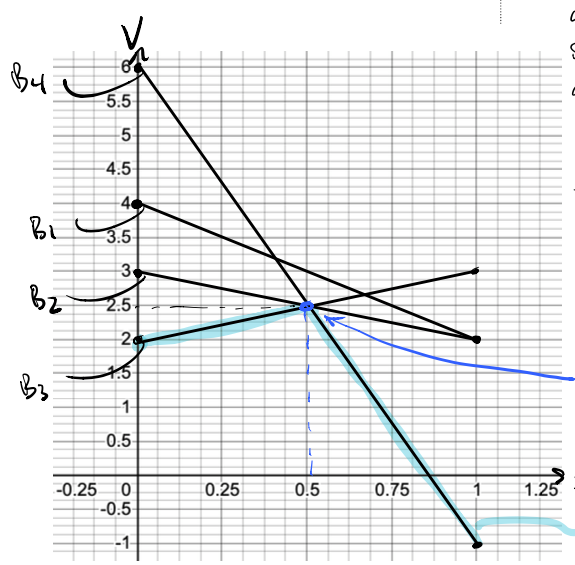
\includegraphics[width = .35\textwidth]{Example_Graph.png}
\end{center}

The graph should have the blue highlighted part of the lines highlighted as well with the value of the game plotted as a point.  

\item Create a \texttt{py} file that uses \texttt{linprog} to solve for all possible coalitions for the following three person zero-sum game: 

\begin{center}
\hspace{-2cm}
\def\arraystretch{2}%
\begin{tabular}{l  c c || c c |}
& \multicolumn{2}{c}{{\underline{$R_1$}}} & \multicolumn{2}{c}{{\underline{$R_2$}}}   \\
& $C_1$ & $C_2$ & $C_1$ & $C_2$   \\ \hline
$L_1$ & $(1,1,-2)$ &  $(-4,3,1)$  &  $(3,-2,-1)$  &  $(-6,-6,12)$   \\
$L_2$ & $(2,-4,2)$ &  $(-5,-5,10)$  &  $(2,2,-4)$  &  $(-2,3,-1)$ \\\hline
\end{tabular}
\end{center}\vspace{.5cm}

The code should implement your code from the Problem 2, and output the graph for each possible coalition. 

\end{enumerate}







































\end{document}